\documentclass{beamer}
\usepackage[utf8]{inputenc}
\usepackage{xcolor}
\usepackage{hyperref}
\usepackage{graphicx}
\usepackage{tikz}
\usetikzlibrary{shapes,fit,positioning,calc,trees}
\usepackage{bbding} % For \HandRight
\usepackage{fancyvrb} % For \UseVerb \SaveVerb

\usetheme{Madrid}
\usecolortheme{default}

% Command that embeds a hand pointing to the right in a href label
\newcommand{\hrefhand}[2]{\raisebox{-0.4ex}{\HandRight}\,\href{#1}{#2}}

\title{COMP3320 Introduction to OpenGL}
\author{Alex Biddulph}
\institute{
    The University of Newcastle, Australia
}
\date{Semester 2, 2021}

\begin{document}

\begin{frame}
    \titlepage
\end{frame}

\begin{frame}{Introduction to OpenGL}
    \begin{itemize}
        \item This lecture series aims at providing a brief overview of OpenGL and associated libraries
        \item A series of C++ code examples are also provided
        \item The code example try to provide modern C++ wrappers around the C libraries in order to simplify the code
    \end{itemize}
\end{frame}

\setbeamercovered{invisible}
\begin{frame}{Libraries}
    The following libraries are used or have a wrapper in the code examples
    \begin{table}
        \centering
        \begin{tabular}{l|l}
            Library                                                                    & Description                                                       \\
            \hline
            \hline
            \hrefhand{https://opengl.org}{\color{blue}OpenGL}                          & For all of our 3D graphics needs                     \onslide<2-> \\
            \hrefhand{https://www.glfw.org}{\color{blue}GLFW}                          & Window and input management                          \onslide<3-> \\
            \hrefhand{https://glad.dav1d.de}{\color{blue}GLAD}                         & OS-specific library abstraction for OpenGL functions \onslide<4-> \\
            \hrefhand{https://glm.g-truc.net/0.9.9/index.html}{\color{blue}GLM}        & OpenGL mathematics library                           \onslide<5-> \\
            \hrefhand{https://www.lonesock.net/soil.html}{\color{blue}SOIL}            & For loading texture files                            \onslide<6-> \\
            \hrefhand{https://www.assimp.org}{\color{blue}Assimp}                      & For loading 3D models                                \onslide<7-> \\
            \hrefhand{https://openal.org}{\color{blue}OpenAL}                          & For all of our 3D audio needs  \onslide<8->                       \\
            \hrefhand{http://libsndfile.github.io/libsndfile/}{\color{blue}libsndfile} & For loading audio files        \onslide<9->                       \\
        \end{tabular}
    \end{table}
\end{frame}

\begin{frame}[fragile]{Github Repository}
    All code examples can be found at the following \hrefhand{https://github.com/Bidski/COMP3320}{\color{blue}Github repository}
    \begin{figure}
        \centering
        \scalebox{1.00}{
            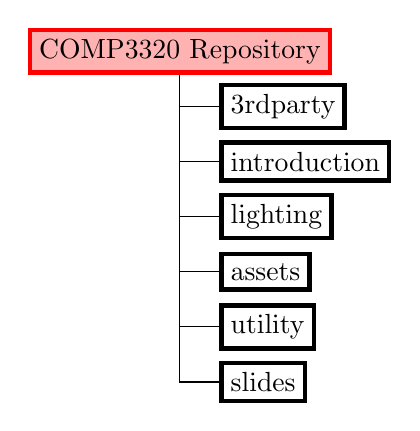
\begin{tikzpicture}[%
                    every node/.style={draw=black,ultra thick,anchor=west},
                    selected/.style={draw=red,fill=red!30},
                    optional/.style={dashed,fill=gray!50},
                    grow via three points={one child at (0.5,-0.7) and
                            two children at (0.5,-0.7) and (0.5,-1.4)},
                    edge from parent path={(\tikzparentnode.south) |- (\tikzchildnode.west)}]
                \node [selected] {COMP3320 Repository}
                child { node {3rdparty}}
                child { node {introduction}}
                child { node {lighting}}
                child { node {assets}}
                child { node {utility}}
                child { node {slides}};
            \end{tikzpicture}
        }
    \end{figure}
\end{frame}

\begin{frame}[fragile]{Github Repository}
    \begin{figure}
        \centering
        \scalebox{0.65}{
            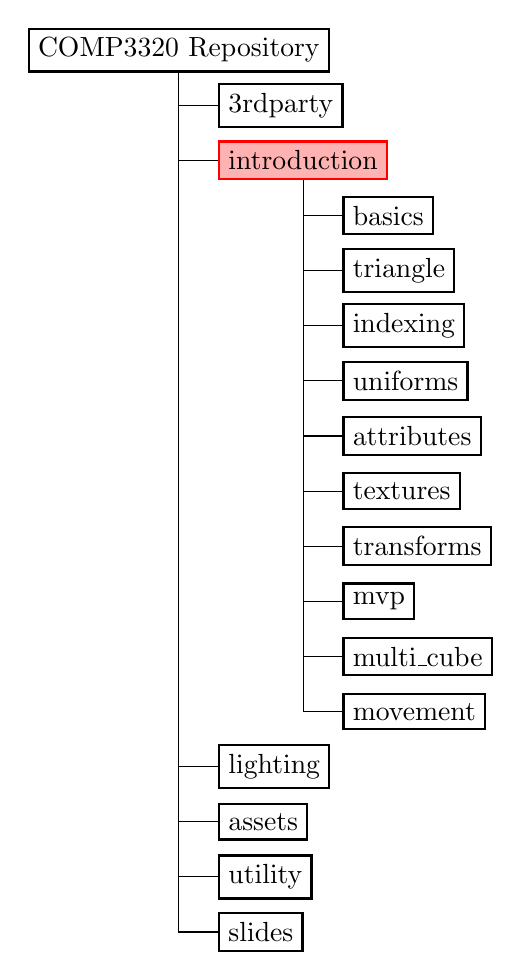
\begin{tikzpicture}[%
                    every node/.style={draw=black,thick,anchor=west},
                    selected/.style={draw=red,fill=red!30},
                    optional/.style={dashed,fill=gray!50},
                    grow via three points={one child at (0.5,-0.7) and
                            two children at (0.5,-0.7) and (0.5,-1.4)},
                    edge from parent path={(\tikzparentnode.south) |- (\tikzchildnode.west)}]
                \node {COMP3320 Repository}
                child { node {3rdparty}}
                child { node [selected] {introduction}
                        child { node {basics}}
                        child { node {triangle}}
                        child { node {indexing}}
                        child { node {uniforms}}
                        child { node {attributes}}
                        child { node {textures}}
                        child { node {transforms}}
                        child { node {mvp}}
                        child { node {multi\_cube}}
                        child { node {movement}}
                    }
                child [missing] {}
                child [missing] {}
                child [missing] {}
                child [missing] {}
                child [missing] {}
                child [missing] {}
                child [missing] {}
                child [missing] {}
                child [missing] {}
                child [missing] {}
                child { node {lighting}}
                child { node {assets}}
                child { node {utility}}
                child { node {slides}};
            \end{tikzpicture}
        }
    \end{figure}
\end{frame}

\begin{frame}[fragile]{Github Repository}
    \begin{figure}
        \centering
        \scalebox{1.00}{
            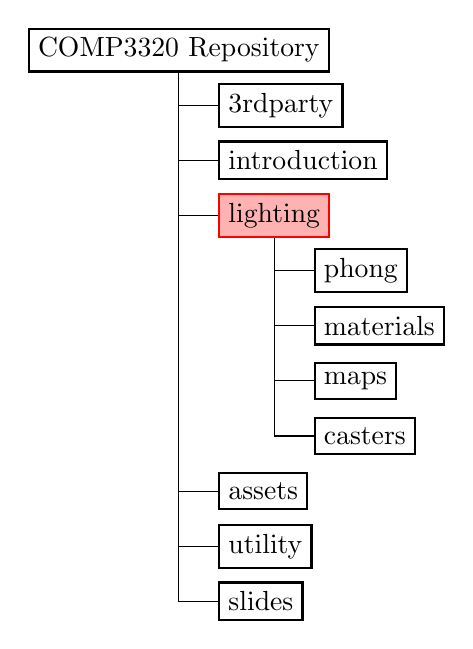
\begin{tikzpicture}[%
                    every node/.style={draw=black,thick,anchor=west},
                    selected/.style={draw=red,fill=red!30},
                    optional/.style={dashed,fill=gray!50},
                    grow via three points={one child at (0.5,-0.7) and
                            two children at (0.5,-0.7) and (0.5,-1.4)},
                    edge from parent path={(\tikzparentnode.south) |- (\tikzchildnode.west)}]
                \node {COMP3320 Repository}
                child { node {3rdparty}}
                child { node {introduction}}
                child { node [selected] {lighting}
                        child { node {phong}}
                        child { node {materials}}
                        child { node {maps}}
                        child { node {casters}}
                    }
                child [missing] {}
                child [missing] {}
                child [missing] {}
                child [missing] {}
                child { node {assets}}
                child { node {utility}}
                child { node {slides}};
            \end{tikzpicture}
        }
    \end{figure}
\end{frame}

\begin{frame}[fragile]{Github Repository}
    \begin{figure}
        \centering
        \scalebox{1.00}{
            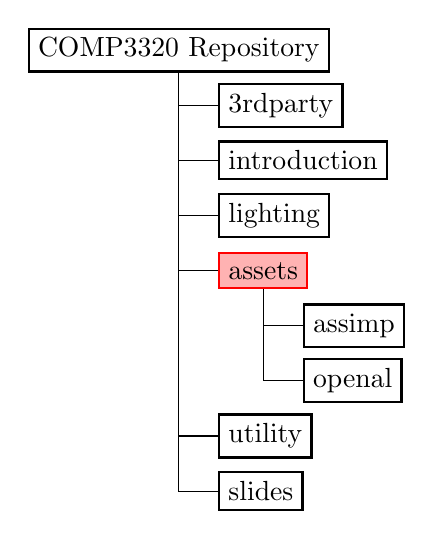
\begin{tikzpicture}[%
                    every node/.style={draw=black,thick,anchor=west},
                    selected/.style={draw=red,fill=red!30},
                    optional/.style={dashed,fill=gray!50},
                    grow via three points={one child at (0.5,-0.7) and
                            two children at (0.5,-0.7) and (0.5,-1.4)},
                    edge from parent path={(\tikzparentnode.south) |- (\tikzchildnode.west)}]
                \node {COMP3320 Repository}
                child { node {3rdparty}}
                child { node {introduction}}
                child { node {lighting}}
                child { node [selected] {assets}
                        child {node {assimp}}
                        child {node {openal}}
                    }
                child [missing] {}
                child [missing] {}
                child { node {utility}}
                child { node {slides}};
            \end{tikzpicture}
        }
    \end{figure}
\end{frame}

\begin{frame}[fragile]{Github Repository}
    \begin{figure}
        \centering
        \scalebox{0.75}{
            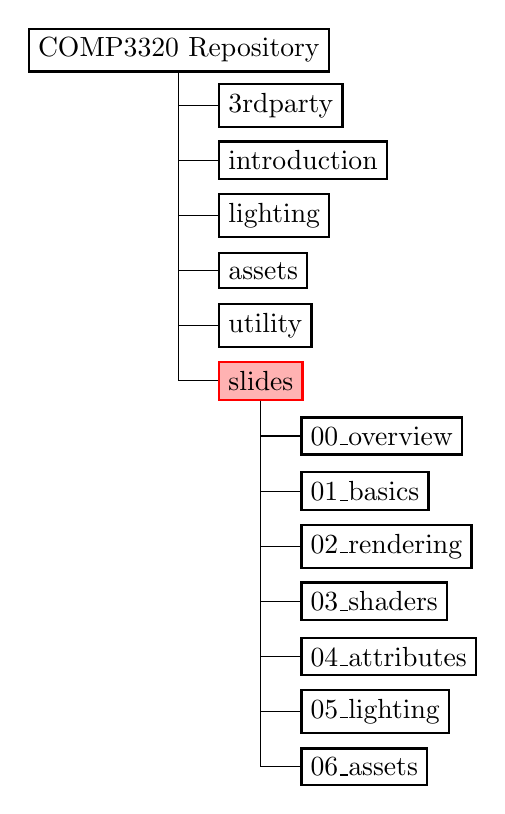
\begin{tikzpicture}[%
                    every node/.style={draw=black,thick,anchor=west},
                    selected/.style={draw=red,fill=red!30},
                    optional/.style={dashed,fill=gray!50},
                    grow via three points={one child at (0.5,-0.7) and
                            two children at (0.5,-0.7) and (0.5,-1.4)},
                    edge from parent path={(\tikzparentnode.south) |- (\tikzchildnode.west)}]
                \node {COMP3320 Repository}
                child { node {3rdparty}}
                child { node {introduction}}
                child { node {lighting}}
                child { node {assets}}
                child { node {utility}}
                child { node [selected] {slides}
                        child {node {00\_overview}}
                        child {node {01\_basics}}
                        child {node {02\_rendering}}
                        child {node {03\_shaders}}
                        child {node {04\_attributes}}
                        child {node {05\_lighting}}
                        child {node {06\_assets}}
                    };
            \end{tikzpicture}
        }
    \end{figure}
\end{frame}

\end{document}
